\documentclass[a4paper,10pt]{article}
\usepackage[utf8]{inputenc}
\usepackage{amsmath}
\usepackage{graphicx}
\numberwithin{equation}{section}

%opening
\title{Quantum 1 HW 4}
\author{Vince Baker}

\begin{document}

\maketitle

\section{Problem 1}
We study phonons with a classical system of springs and masses. 
We have N masses of mass m coupled with springs of spring constant k.
Masses 1 and N are anchored to a wall.\\
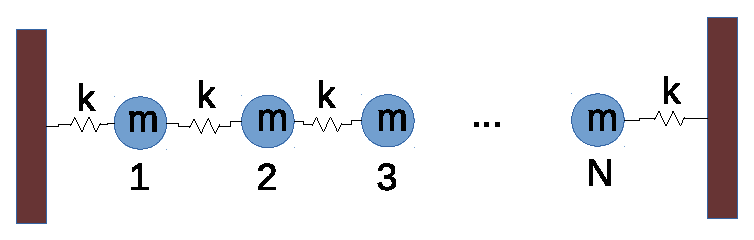
\includegraphics{p1}
\\
We compute the dispersion relation, which is the mode-dependence of the frequency $\omega_{\hat{m}}=\omega_0\times2\sin{\frac{\hat{m}}{N+1}\frac{\pi}{2}}$.
\\ \\
The expected value of the energy in mode j is:
\begin{gather}
 <E_j>=(\bar{n}(j)+\frac{1}{2})\hbar \omega_j,\ \bar{n}=\frac{1}{e^{\beta\hbar \omega_j}-1}
\end{gather}
The total mean thermal energy can be written as a sum of the individual mode terms.
\begin{gather}
 <E>=\sum_j(\bar{n}(j)+\frac{1}{2})\hbar \omega_j
\end{gather}
We can separate the $\bar{n}(j)$ and $\frac{1}{2}$ terms of the sum.
\begin{gather}
 <E>=\sum_j\bar{n}(j)\hbar \omega_j+\sum_j \frac{1}{2}\hbar \omega_j
\end{gather}
The left term depends on the temperature ($\beta=\frac{1}{kT}$), the right term is temperature independent.\\ \\
We expand the left sum:
\begin{gather}
 \sum_j\bar{n}(j)\hbar \omega_j=\sum_j \frac{\hbar \omega_j}{e^{\frac{\hbar \omega_j}{kT}}-1}
\end{gather}


\section{Problem 2}
The temperature-independent zero-point energy is:
\begin{gather}
  <E_{zp}>=\sum_j \frac{1}{2}\hbar \omega_j
\end{gather}
The mode frequencies are $\omega_{\hat{m}}=2\omega_0\sin{\frac{\hat{m}}{N+1}\frac{\pi}{2}}$. We can rewrite this using:
\begin{gather}
 \sum_j\sin\frac{j\frac{\pi}{2}}{N+1}=\frac{1}{2}\frac{\cos \theta+\sin \theta-1}{1-\cos \theta},\ \theta=\frac{\frac{\pi}{2}}{N+1}\\
 <E_{zp}>=\hbar\omega_0\frac{\cos \theta+\sin \theta-1}{1-\cos \theta}
\end{gather}
We can now calculate the zero-point energy of both the complete 100-atom system and the sum of individual sub-systems.
We take $m=k=\hbar=1$ to simplify the calculations. We now calculate zero-point energies for different values of N.\\ \\
The energy to fix the mass at position 50 is:
\begin{equation}
 <E_{zp}(100)>-<E_{zp}(50)>-<E_{zp}(49)>=1.00778
\end{equation}
\\
The energy to fix the mass at position 25 is:
\begin{equation}
 <E_{zp}(100)>-<E_{zp}(24)>-<E_{zp}(75)>=1.0113
\end{equation}
\\ 
The energy to fix the mass at position 24 is:
\begin{equation}
 <E_{zp}(100)>-<E_{zp}(23)>-<E_{zp}(76)>=1.0117
\end{equation}
\\
It requires additional energy $-3.92e^{-4}$ to hold mass 24 fixed compared to mass 25. 
With $F=-\nabla V$, the gradient of the energy is the energy difference divided by the separation between masses, so $F_{25}=3.92e^{-4}/\ell$ and the force is toward the left wall.

\section{Problem 3}
Debye's theory of lattice vibrations estimates the number of normal modes within $d\omega$ of $\omega$ to be $K4\pi\omega ^2 d\omega$.
In a 3-D lattice of N atoms there will be 3N normal modes. If the highest Debye normal mode is $\omega_d$, then we can calculate the constant K:
\begin{gather}
 \int_{0}^{\omega_d}K4\pi\omega ^2 d\omega=3N\\
 K=\frac{9N}{4\pi \omega_{d}^{3}}
\end{gather}


\end{document}
